\documentclass[a4paper,10pt]{book}

\usepackage[utf8]{inputenc}
\usepackage{amsmath}
\usepackage{amsfonts}
\usepackage{amssymb}
\usepackage{amsthm}
\usepackage[czech]{babel}
\usepackage{fontenc}
\usepackage{fancyhdr} %zahlavi a zapati
\usepackage{a4wide} % širší stránka
\usepackage{float} % obrázky na jedno místo
\usepackage{tikz}
\usepackage{listings}  % for source code (python\dots)
\usetikzlibrary {positioning}
\usepackage{tkz-euclide}
\usetkzobj{all}
\usetikzlibrary{calc,patterns}
\usetikzlibrary{intersections}
\usetikzlibrary{arrows,automata,shapes,quotes,decorations.markings}
\usepackage{tikz-3dplot}
\usepackage{newclude} % include bez clearpage
\usepackage{graphicx}
\usepackage{minted} % python code
\usepackage{multicol}
\usepackage{hyperref}
\usepackage[all]{hypcap}
\usepackage[parfill]{parskip}

% umožní vícestránkový align
\allowdisplaybreaks

% rejstřík
\usepackage{makeidx}
\makeindex

\title{Řešená cvičení z Matematické analýzy I}
\author{Jaroslav Hančl, Karel Král, Ondřej Pangrác}
\date{\today}

% theory macro
\newcommand{\theory}[1]{
	%\begin{center}
		%\line(1,0){250}
	%\end{center}
	%\newline % tady to dělá neplechu
	#1
}

\begin{document}
% Definitions
\newtheorem{theorem}{Věta}
\newtheorem{lemma}[theorem]{Lemma}
\newtheorem{conjecture}[theorem]{Domněnka}
\newtheorem{observation}[theorem]{Pozorování}
\newtheorem{corollary}[theorem]{Důsledek}
\newtheorem*{definition}{Definice}
%\theoremstyle{definition}\newtheorem*{define}{Definice}

 \maketitle

 \vskip 1cm

 Tento text není určen k šíření.
 Všechny chyby v tomto textu jsou samozřejmě záměrné. Reportujte je prosím na adresu
 {\tt kralka@iuuk.mff.cuni\ldots}.

 \vskip 2cm
 \tableofcontents

 \newcommand{\dif}{\, \mathrm{d}} % put at the beginning of document
 \newcommand{\id}{\, \mathrm{id}} % put at the beginning of document
 \newcommand{\sgn}{\, \mathrm{sgn}} % put at the beginning of document
 \newcommand{\med}{\, \mathrm{med}} % put at the beginning of document
 \newcommand{\conv}{\, \mathrm{conv}} % put at the beginning of document
 \newcommand{\supp}{\, \mathrm{Supp}} % put at the beginning of document
 \newcommand{\Ker}{\, \mathrm{Ker}} % put at the beginning of document
 \renewcommand{\Im}{\, \mathrm{Im}} % put at the beginning of document
 \newcommand{\R}{\, \mathcal{R}} % put at the beginning of document
 % nastavíme použití toho stylu
  %\pagestyle{fancy}
 % fakt hloupý nápad, když chci rejstřík
 %\pagenumbering{gobble} % bez čísel stránek

	\eject

\chapter{Zadání}
	% solution macro, this does NOT prints the solution
	\newcommand{\solution}[1]{}
	\newcommand{\exercise}[2]{ % file, label
		\input{#1}

		Řešení: \ref{sol:#2}
	}
	\section[1. Cvičení]{Cvičení}
 \include*{s1}
	\section[2. Cvičení]{Cvičení}
 \include*{s2}
	\section[3. Cvičení]{Cvičení}
 \include*{s3}
	\section[4. Cvičení]{Cvičení}
 \include*{s4}
	\section[5. Cvičení]{Cvičení}
 \include*{s5}
	\section[6. Cvičení]{Cvičení}
 \include*{s6}
	\section[7. Cvičení]{Cvičení}
 \include*{s7}
	\section[8. Cvičení]{Cvičení}
 \include*{s8}

\chapter{Tahák}
	\section{Základní vlastnosti funkcí}
	\section{Logika}
		Negace výroků:
\begin{multicols}{2}
\begin{enumerate}
	\item  $\neg (\neg A) \equiv A$
	\item  $\neg (A \wedge B) \equiv (\neg A) \vee (\neg B)$
	\item  $\neg (A \vee B) \equiv (\neg A) \wedge (\neg B)$
	\item  $\neg (A \Rightarrow B) \equiv A \wedge (\neg B)$
	\item  $\neg (A \Leftrightarrow B) \equiv A \Leftrightarrow (\neg B)$
	\item  $\neg \left( \forall x \colon \varphi(x) \right) \equiv \exists x \colon \neg \varphi(x)$
	\item  $\neg \left( \exists x \colon \varphi(x) \right) \equiv \forall x \colon \neg \varphi(x)$
\end{enumerate}
\end{multicols}
Pozor na ``existuje právě jedno'': $\neg \left( \exists! x \colon \varphi(x) \right) \equiv \left( \forall x \colon \neg \varphi(x) \right) \vee \left( \exists x \exists y \colon x \neq y \wedge \varphi(x) \wedge \varphi(y) \right)$


	\section{Limity}
		\begin{definition}
	Nechť $(a_a) \subset \mathbb{R}, a \in \mathbb{R}$.
	Číslo $a$ je limitou posloupnosti $(a_n)$, psáno $\lim a_n = \lim_{n \rightarrow \infty} a_n = a$, když
	$$\forall \varepsilon > 0 \  \exists n_0 \in \mathbb{N} \  \forall n > n_0 \colon |a_n - a| < \varepsilon.$$
	\label{def:limita_vlastni}
\end{definition}


		\begin{theorem}[Bolzano-Weierstrass (BW)]
	Každá posloupnost $(a_n)_{n=1}^{\infty}$ má podposloupnost $(b_n)_{n=1}^{\infty}$, která je monotónní.
	\label{thm:bolzano_weierstrass}
\end{theorem}

\begin{theorem}[(EDL)]
	$\lim_{n \rightarrow \infty} a_n = a \Leftrightarrow \lim_{n \rightarrow \infty}(a_n - a) = 0 \Leftrightarrow \lim_{n \rightarrow \infty}|a_n - a| = 0$
	speciálně $\lim_{n \rightarrow \infty} a_n = 0 \Leftrightarrow \lim_{n \rightarrow \infty} |a_n| = 0$.
	\label{thm:edl}
\end{theorem}

\begin{theorem}[Věta o limitě podposloupnosti (VOVP)]
	Nechť $\lim_{n \rightarrow \infty} a_n = a \in \mathbb{R} \cup \left\{ -\infty, +\infty \right\}$ a $(b_n)$ je posloupnost vybraná z $(a_n)$.
	Pak $\lim_{n \rightarrow \infty} a_n = \lim_{n \rightarrow \infty} b_n$.
	\label{thm:veta_o_vybrane_posloupnosti}
\end{theorem}

\begin{theorem}[Věta o aritmetice limit (VOAL)]
	Nechť $a, b \in \mathbb{R} \cup \{\pm \infty \}$ a posloupnosti $(a_n), (b_n)$ splňují $\lim a_n = a$ a $\lim b_n = b$.
	Potom
	\begin{align*}
			\lim_{n \rightarrow \infty}(a_n \pm b_n) &= \lim_{n \rightarrow \infty} a_n \pm \lim_{n \rightarrow \infty} b_n = a \pm b \\
			\lim_{n \rightarrow \infty}a_nb_n &= \lim_{n \rightarrow \infty} a_n \cdot \lim_{n \rightarrow \infty} b_n = ab \\
			\lim_{n \rightarrow \infty}\frac{a_n}{b_n} &= \frac{\lim_{n \rightarrow \infty} a_n}{\lim_{n \rightarrow \infty} b_n} = \frac{a}{b} \mbox{ pro } b \not= 0
	\end{align*}
	pokud má pravá strana těchto rovností smysl.
	\begin{itemize}

			\item Smysl dává:
				$$t + \infty = \infty + t = \infty$$
				$$t - \infty = -\infty + t = -\infty$$
				$$t / \pm \infty = 0$$
				$$\infty + \infty = \infty \cdot \infty = \infty$$
				$$-\infty - \infty = -\infty$$
				$$(-\infty) \cdot (- \infty) = \infty$$
				kde $t \in \mathbb{R}$.

				Pro $t \in (0, \infty]$ máme
				$$t \cdot \infty = \infty \cdot t = \infty$$
				$$t \cdot (-\infty) = (-\infty) \cdot t = -\infty$$
				
				Pro $t \in [-\infty, 0)$ máme
				$$t \cdot \infty = \infty \cdot t = -\infty$$
				$$t \cdot (-\infty) = (-\infty) \cdot t = \infty$$

			\item Smysl nedává (a tedy nemůžeme použít tuto větu přímo, ale musíme dál přemýšlet -- laicky řečeno tady záleží jak jsou ta nekonečna velká, případně jak malé jsou ty nuly):
				$$\pm \infty / \pm \infty$$
				$$\mbox{cokoliv}/0$$
				$$\infty - \infty$$
				$$-\infty - (-\infty)$$
				$$0 \cdot (\pm \infty)$$

	\end{itemize}
	\label{thm:veta_o_aritmetice_limit}
\end{theorem}

\begin{theorem}[Věta o dvou policajtech]
	Nechť posloupnosti $(a_n), (b_n), (c_n) \subset \mathbb{R}$ splňují, že
	$$\underset{n \rightarrow \infty}{\lim} a_n = \underset{n \rightarrow \infty}{\lim} b_n = a \in \mathbb{R}$$
	a nechť existuje $n_0 \in \mathbb{N}$ takové, že pro každé $n > n_0$ platí $a_n \leq c_n \leq b_n$.
	Pak $(c_n)$ konverguje a navíc $\underset{n \rightarrow \infty}{\lim} c_n = a$.
	\label{thm:dva_policajti}
\end{theorem}

\begin{theorem}[Násobení limitní nulou (VOSON)]
	Nechť posloupnost $(a_n)$ je omezená a posloupnost $(b_n)$ konverguje k nule, pak $\lim_{n \rightarrow \infty} a_n \cdot b_n = 0$.
	\label{thm:nasobeni_limitni_nulou}
\end{theorem}

\begin{theorem}
	Nechť $(a_n) \subset (0, \infty)$ je posloupnost kladných reálných čísel a nechť $N \in \mathbb{N}$ je takové, že $\exists q \in [0,1)$ že pro každé přirozené $n \geq N$ platí:
	$$\frac{a_{n+1}}{a_n} \leq q < 1.$$

	Pak:
	\begin{enumerate}
		\item  Pro každé přirozené $n \geq N$ platí $a_n \leq a_N q^{n - N}$ (matematickou indukcí)
		\item  v důsledku čehož: $\underset{n\rightarrow\infty}{\lim} a_n = 0$.
	\end{enumerate}

	Pozor na to, že existuje posloupnost \textbf{kladných} reálných čísel $(b_n)$ taková, že:
	\begin{itemize}
		\item  $b_n > 0$ pro všechna přirozená $n$
		\item  $\frac{b_{n+1}}{b_n} < 1$
		\item  $\underset{n\rightarrow\infty}{\lim} b_n > 0$
	\end{itemize}
	\label{thm:podilove_kriterium_o_konvergenci_k_nule}
\end{theorem}

\begin{theorem}
	Pro libovolné $a \in (0,1)$ platí, že $\underset{n\rightarrow\infty}{\lim} n^a = \infty$.

	Pozor, že například $\underset{n\rightarrow\infty}{\lim} \sqrt[n]{n} = \underset{n\rightarrow\infty}{\lim} \left( n^{1/n} \right) = 1$.
	Takže tato věta nelze přímo použít na nekonstatní odmocniny.
	\label{thm:veta_o_limite_odmocniny}
\end{theorem}


	\section{Hromadné body}
	  \begin{definition}[Hromadný bod]
	Reálné číslo $\alpha$ nazveme hromadným bodem posloupnosti $(a_n)$, pokud existuje posloupnost $(b_n)$ vybraná z $(a_n)$, která má limitu $\alpha$.
	Množinu všech hromadných bodů posloupnosti $(a_n)$ značíme $H(a_n)$.
	Dále definujme nejmenší a největší limitu posloupnosti
	$$
			\liminf_{n \rightarrow \infty} a_n = \min(H) \qquad \mbox{a} \qquad \limsup_{n \rightarrow \infty} a_n = \max(H).
	$$ 
	\label{def:hromadny_bod}
\end{definition}

\begin{theorem}[Základní vlastnosti množiny hromadných bodů]
	Množina $H(a_n)$ je neprázdná a je jednobodová právě, tehdy když $(a_n)$ má limitu.
	Hodnoty $\liminf$ a $\limsup$ vždy existují a pokud je posloupnost omezená, tak jsou to vlastní hodnoty.
	(Podívejte se na ekvivalenty těchto vlastností do poznámek z přednášky.)
	\label{thm:vety_o_hromadnych_bodech}
\end{theorem}


	\section{Řady}
	  \begin{definition}[Definice konvergence řad]
	Říkáme, že řada $\sum a_n$ konverguje, pokud konverguje posloupnost částečných součtů $(s_n)$ zadaná vztahem $s_n = a_1 + a_2 + \dots + a_n$. 
	\label{def:konvergentni_rada}
\end{definition}

\subsection{Základní řady:}

\begin{equation}
	\sum_{n=1}^{\infty} q^n =
	\begin{cases}
		\frac{1}{1-q}			& \text{pro } |q| < 1, \\
		+\infty 	   			& \text{pro } q \geq 1, \\
		\text{neexistuje} & \text{pro } q \leq -1,
	\end{cases}
	\label{eq:rada_q_na_n}
\end{equation}

\begin{equation}
	\sum_{n=1}^{\infty} n^{-\alpha} =
	\begin{cases}
		\text{konverguje}  & \text{pro } \alpha > 1, \\
		\text{diverguje}   & \text{pro } \alpha \leq 1.
	\end{cases}
	\label{eq:rada_n_na_alpha}
\end{equation}


\subsection{Další kritéria na konvergenci řad:}

\begin{theorem}[Další kritéria konvergence řad]
	Nechť $\sum a_n$, $\sum b_n$ jsou řady s nezápornými koeficienty. 
	\begin{itemize}

		\item[(NPK)] \emph{Nutná podmínka konvergence:} \label{thm:konvergence_kriterium_nutna_podminka_konvergence}
			Pokud řada $\sum a_n$ konverguje, pak $\lim a_n = 0$.

		\item[(SK)] \label{thm:konvergence_kriterium_SK}
			Pokud $a_n < b_n$ a $\sum b_n$ konverguje, pak i $\sum a_n$ konverguje. \\ 
			Pokud $a_n < b_n$ a $\sum a_n$ diverguje, pak i $\sum b_n$ diverguje.

		\item[(LSK)] \label{thm:konvergence_kriterium_LSK}
			Definujme $\lim \frac{a_n}{b_n} = \ell$. Pak pro $0 < \ell < \infty$ platí, že $\sum a_n$ konverguje $\Leftrightarrow$ $\sum b_n$ konverguje.
	\end{itemize}
	\label{thm:konvergence_rad}
\end{theorem}


	\section{Limity funkcí}
	  \begin{definition}[Okolí]
	\emph{Okolí bodu} $a \in \mathbb{R}$ (přesněji $\delta$-okolí bodu $a$, kde $\delta > 0$) je interval $U(a, \delta) = (a - \delta, a + \delta)$, neboli
	$$U(a, \delta) = \left\{ x \in \mathbb{R} \mid |x - a| < \delta \right\}.$$

	\emph{Okolí nekonečna} definujeme jako $U(+\infty, \delta) = (1/\delta, +\infty)$, $U(-\infty, \delta) = (-\infty, 1/\delta)$.

	\emph{Pravé okolí} $U^+(a, \delta) = [a, a + \delta)$, \emph{levé okolí} je symetricky $U^-(a, \delta) = (a-\delta, a]$.

	\emph{Prstencové okolí} je okolí bez toho bodu, tedy $P(a, \delta) = U(a, \delta) \setminus \left\{ a \right\}$.
	\label{def:okoli}
\end{definition}


	  \begin{definition}[Limita funkce]
	Řekneme, že funkce $f$ má v bodě $a \in \mathbb{R}$ limitu $A \in \mathbb{R}$ pokud 
	$$\forall \varepsilon>0 \ \exists \delta>0 \colon x \in P(a, \delta) \Rightarrow  f(x) \in U(A, \varepsilon) \ .$$
	Zapisujeme $\lim_{x \rightarrow a} f(x) = A$.
	\label{def:limita_funkce}
\end{definition}


	  \begin{theorem}[Aritmetika limit funkcí]
	Nechť $a, A, B \in \mathbb{R}^*$,
	nechť $f, g$ jsou funkce definované na nějakém prstencovém okolí $P(a, \Delta)$ bodu $a$,
	nechť platí $\underset{x \rightarrow a}{\lim} f(x) = A$, $\underset{x \rightarrow a}{\lim} g(x) = B$.
	Potom:
	\begin{enumerate}

		\item  $\underset{x \rightarrow a}{\lim} f(x) + g(x) = A + B$, je-li tento součet definovaný
			\label{thm:aritmetika_limit_funkci:soucet}

		\item  $\underset{x \rightarrow a}{\lim} f(x) g(x) = A \cdot B$, je-li tento součin definovaný
			\label{thm:aritmetika_limit_funkci:soucin}

		\item  Nechť je navíc $g$ na nějakém prstencovém okolí bodu $a$ nenulová, pak
			$\underset{x \rightarrow a}{\lim} f(x) / g(x) = A / B$, je-li tento podíl definovaný
			\label{thm:aritmetika_limit_funkci:podil}

	\end{enumerate}
	\label{thm:aritmetika_limit_funkci}
\end{theorem}


	  \begin{theorem}[Limita složené funkce]
	Nechť $A, B, C \in \mathbb{R}^*$,
	nechť $g(x)$ je funkce splňující
	$$\lim_{x \rightarrow A} g(x) = B,$$ 
	a $f(x)$ je funkce splňující
	$$\lim_{x \rightarrow B} f(x) = C.$$ 
	Navíc nechť je splněna aspoň jedna z následujících podmínek:
	\begin{itemize}

		\item[\textbf{P1}]  Funkce $f(x)$ je spojitá v $B$ (tedy $f(B) = \underset{x \rightarrow B}{\lim} f(x) = C)$.
		
		\item[\textbf{P2}]  Na nějakém prstencovém okolí $P(A, \eta)$ funkce $g(x)$ nenabývá hodnotu $B$, tj. $B \not\in g(P(A, \eta))$.

	\end{itemize}
	Pak
	$$\lim_{x \rightarrow A} f(g(x)) = C.$$
	\label{thm:limita_slozene_fce}
\end{theorem}


	\section{Derivace}
	  \begin{definition}
	Nechť $f \colon M \rightarrow \mathbb{R}$, $b \in M$, $U(b, \delta) \subseteq M$ pro nějaké $\delta > 0$.
	Derivace funkce $f$ v bodě $b$ je limita:
	$$f'(b) = \lim_{h \rightarrow 0} \frac{f(b + h) - f(b)}{h}$$
	\label{def:derivace}
\end{definition}

\begin{figure}[h]
	\centering
	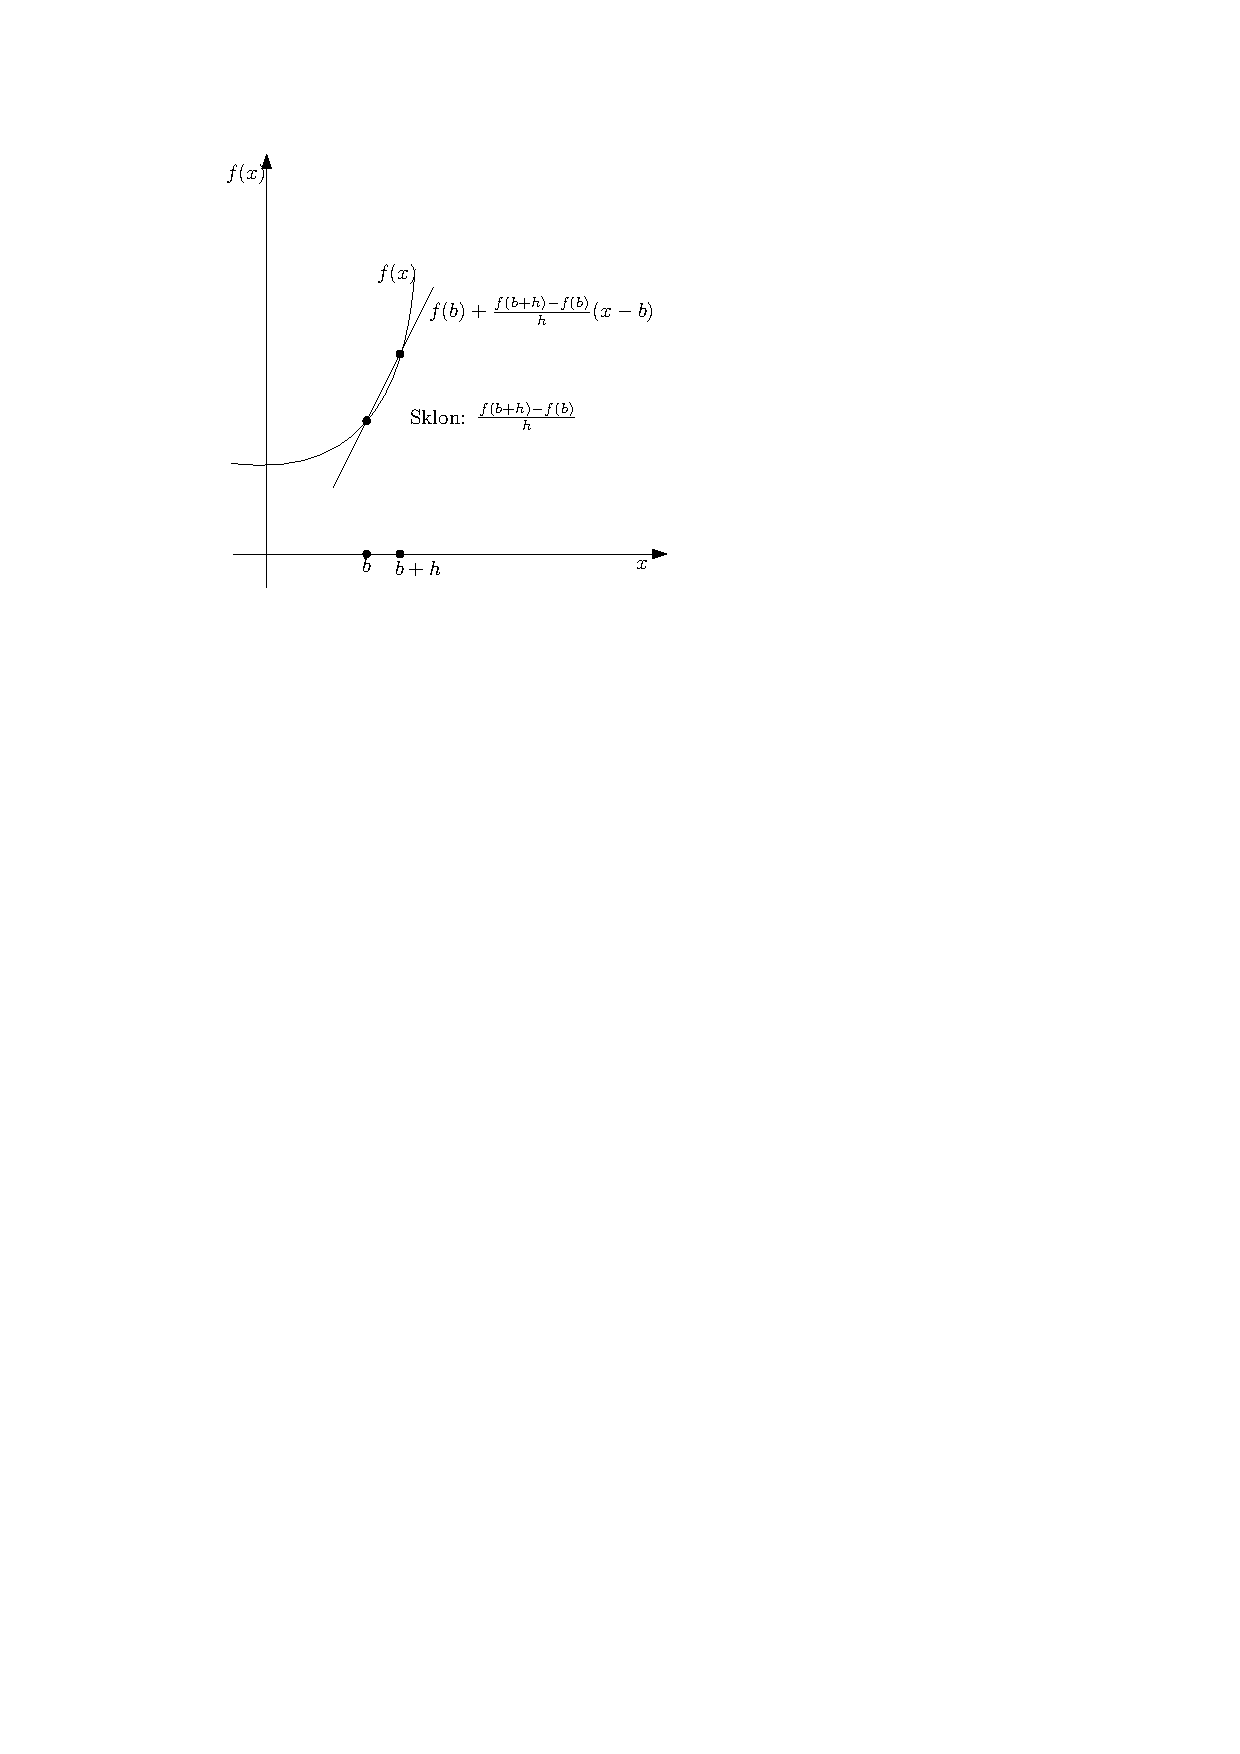
\includegraphics{tahaky/fig/derivace.pdf}
	\caption{Definice derivace v obrázku pro pevné $h$}
	\label{fig:def:derivace}
\end{figure}



	  \begin{theorem}
	O derivacích víte následující:
	\begin{enumerate}
		\item  $c' = 0$ (derivace konstanty je nula) \label{poucka:derivace_konstanty}
		\item  $(x^k)' = k x^{k-1}$ pro libovolné $k \in \mathbb{R}$ kdykoliv je toto definováno (bacha na dělení nulou při derivaci $(x^{1/2})' = \frac{1}{\sqrt{x}}$) \label{poucka:derivace_monomu}
		\item  $\sin'(x) = \cos(x)$ \label{poucka:derivace_sin}
		\item  $\cos'(x) = -\sin(x)$ \label{poucka:derivace_cos}
		\item  $\ln'(x) = 1/x$ pro $x>0$ \label{poucka:derivace_ln}
		\item  $\left( \frac{f(x)}{g(x)} \right)' = \frac{f'(x)g(x) - f(x)g'(x)}{g(x)^2}$ kdekoliv $g(x) \neq 0$
		\item  $(e^x)' = e^x$ \label{poucka:derivace_exponencialy}
		\item  Derivace je lineární operátor, tedy $(\alpha f + \beta g)'(x) = \alpha f'(x) + \beta g'(x)$ pokud je pravá strana definována \label{poucka:derivace_je_linearni_operator}
		\item  $(f\cdot g)'(x) = f'(x) g(x) + f(x) g'(x)$ pokud je pravá strana definována a $f$ nebo $g$ je spojitá \label{poucka:derivace_soucinu}
		\item  $(f\circ g)'(x) = f'(g(x)) g'(x)$ pokud je pravá strana definována, $g, f$ mají derivaci a $g$ je spojitá \label{poucka:derivace_slozene_fce}
	\end{enumerate}
	\label{thm:poucky_o_derivacich}
\end{theorem}



\chapter{Řešení}
	% solution macro, this prints the solution
	\renewcommand{\solution}[1]{
		\emph{Řešení:}
		#1
	}
	\renewcommand{\exercise}[2]{ % file, label
		\label{sol:#2}
		\input{#1}
		\newpage
	}
	\section[1. Cvičení]{Cvičení}
 \include*{s1}
	\section[2. Cvičení]{Cvičení}
 \include*{s2}
	\section[3. Cvičení]{Cvičení}
 \include*{s3}
	\section[4. Cvičení]{Cvičení}
 \include*{s4}
	\section[5. Cvičení]{Cvičení}
 \include*{s5}
	\section[6. Cvičení]{Cvičení}
 \include*{s6}
	\section[7. Cvičení]{Cvičení}
 \include*{s7}
	\section[8. Cvičení]{Cvičení}
 \include*{s8}

\chapter{Řešení vybraných domácích úkolů}

\begin{enumerate}
	\item  \exercise{homework/charakterizace_kdy_omezena_nema_limitu.tex}{charakterizace_nema_limitu}
	%\item  \exercise{homework/rekurentni.tex}{rekurentni}
\end{enumerate}

\end{document}
